\documentclass[12pt]{article}
\usepackage{times,amsmath,amsthm,latexsym,fullpage}

% for tikz (drawing automata)
\usepackage{pgf}
\usepackage{tikz}
\usetikzlibrary{arrows,automata}

\setlength{\parskip}{.1in}

\renewcommand{\baselinestretch}{1.1} 

\theoremstyle{definition}
\newtheorem*{solution}{Solution}


\begin{document}

\begin{center}
CSCE 433 / CSCE 627:  Homework 2 \\
\end{center}

\begin{itemize}
\item Don't forget to review the general instructions (on Piazza)!

\item {\bf Due Wed, Feb 14, 11:30 AM}
\end{itemize}

\begin{enumerate}

\item (20 points) Give a regular grammar for each of the following
languages:
  \begin{enumerate}
  \item all strings over $\{a,b\}$ that do not contain $ab$
\begin{solution}
	$G = (\{S,A\}, \{a,b\}, R, S)$ where the rules in $R$ are as follows\\ 
	$S \rightarrow bS | bA | aA | b | a | \epsilon$ \\ 
	$A \rightarrow aA |a$ \\
	\end{solution}
  \item all binary strings that contain at least three 1's
  \begin{solution}
	$G = (\{S,A,B,C\}, \{0,1\}, R, S)$ where the rules in $R$ are as follows\\ 
	$S \rightarrow 0S | 1A $ \\ 
	$A \rightarrow 1B | 0A$ \\
	$B \rightarrow 1C | 0B$ \\
	$C \rightarrow 0C | 1C | 0 | 1$
	\end{solution}
  \item all binary strings $w$ such that every odd position in $w$ is a 1
    \begin{solution}
	$G = (\{S, A\}, \{0,1\}, R, S)$ where the rules in $R$ are as follows\\ 
	$S \rightarrow 1A | 1 | \epsilon$ \\ 
	$A \rightarrow 0S| 1S | 0 | 1$ 
	\end{solution}
  \item (CSCE 433 students only) all strings over $\{a,b\}$ that contain
        at least one $a$ and every $a$ is immediately followed by at least
        on $b$
	\begin{solution}
	$G = (\{S,A,B\}, \{a,b\}, R, S)$ where the rules in $R$ are as follows\\ 
	$S \rightarrow aA | bB | a$ \\ 
	$A \rightarrow bA | b | bS $ \\
	$B \rightarrow bB | bS | a$
	\end{solution}
  \item (CSCE 627 students only) all strings over $\{a,b\}$ with an
        even number of $a$'s and an odd number of $b$'s
	\begin{solution}
	$G = (\{S,A,B,C\}, \{a,b\}, R, S)$ where the rules in $R$ are as follows\\ 
	$S \rightarrow aA | bB $ \\ 
	$A \rightarrow aS | bC$ \\
	$B \rightarrow aS | bC $ \\
	$C \rightarrow b | bA | aS$ \\
	\end{solution}
  \end{enumerate}

\item (10 points) Use the algorithm given in class (and lecture notes)
to convert the following regular grammar into an NFA:
\begin{align*}
S &\rightarrow aS | aX | a \\
X &\rightarrow bS | aY \\
Y &\rightarrow bS
\end{align*}
\begin{solution}
We are given $G = (\{S,X,Y\},\{a,b\},R,S)$. We define our NFA $N$ as follows: we create a state for each variable plus one finishing state, set the stating state to the one representing our variable $S$, and set the transitions to match the set of rules plus an extra transition from $q_S$ to $q_F$ because we have that S can turn into a single terminal $a$. $$N = (Q=\{q_S,q_X,q_Y,q_F\},\Sigma = \{a,b\},\delta = Q*\Sigma\rightarrow Q,q_S,F=\{q_F\})$$
\begin{center}
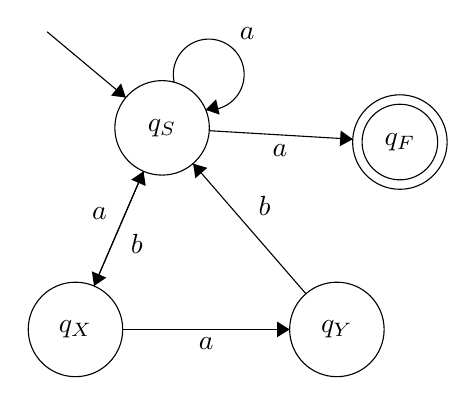
\begin{tikzpicture}[scale=0.2]
\tikzstyle{every node}+=[inner sep=0pt]
\draw [black] (26.9,-29.3) circle (3);
\draw (26.9,-29.3) node {$q_X$};
\draw [black] (43.5,-29.3) circle (3);
\draw (43.5,-29.3) node {$q_Y$};
\draw [black] (47.5,-17.4) circle (3);
\draw (47.5,-17.4) node {$q_F$};
\draw [black] (47.5,-17.4) circle (2.4);
\draw [black] (32.4,-16.5) circle (3);
\draw (32.4,-16.5) node {$q_S$};
\draw [black] (33.169,-13.612) arc (192.81407:-95.18593:2.25);
\draw (37.8,-10.93) node [above] {$a$};
\fill [black] (35.16,-15.35) -- (36.05,-15.66) -- (35.83,-14.69);
\draw [black] (25.1,-10.4) -- (30.1,-14.58);
\fill [black] (30.1,-14.58) -- (29.8,-13.68) -- (29.16,-14.45);
\draw [black] (35.39,-16.68) -- (44.51,-17.22);
\fill [black] (44.51,-17.22) -- (43.74,-16.67) -- (43.68,-17.67);
\draw (39.88,-17.5) node [below] {$a$};
\draw [black] (28.08,-26.54) -- (31.22,-19.26);
\fill [black] (31.22,-19.26) -- (30.44,-19.79) -- (31.36,-20.19);
\draw (30.38,-23.86) node [right] {$b$};
\draw [black] (31.22,-19.26) -- (28.08,-26.54);
\fill [black] (28.08,-26.54) -- (28.86,-26.01) -- (27.94,-25.61);
\draw (28.92,-21.94) node [left] {$a$};
\draw [black] (29.9,-29.3) -- (40.5,-29.3);
\fill [black] (40.5,-29.3) -- (39.7,-28.8) -- (39.7,-29.8);
\draw (35.2,-29.8) node [below] {$a$};
\draw [black] (41.53,-27.03) -- (34.37,-18.77);
\fill [black] (34.37,-18.77) -- (34.51,-19.7) -- (35.27,-19.04);
\draw (38.49,-21.45) node [right] {$b$};
\end{tikzpicture}
\end{center}
\end{solution}

\item (10 points) Use the algorithm given in class (and lecture notes)
to convert the DFA in Exercise 1.21(b) into a regular grammar.

\item (20 points) Use the pumping lemma for regular languages
to show that the following languages are not regular
(you might find it useful to study the solutions in the textbook
to Exercise 1.29, parts (a) and (c)):
  \begin{enumerate}
  \item $\{www | w \in \{a,b\}^*\}$
  \item $\{a^i (ab)^j (ca)^{2i} | i > 0, j > 0 \}$
  \item the set of properly nested parentheses (e.g., includes ``()(())()''
        but not ``)(``)
  \item (CSCE 433 students only) $\{a^n b^m | n < m \}$
  \item (CSCE 627 students only) $\{a^i b^j c^{2j} | i \ge 0, j \ge 0 \}$
  \end{enumerate}

\item (20 points) Problem 1.46, parts (a) and (c).

\end{enumerate}

*** more will be added about context-free languages ***

\end{document}
